\documentclass[12pt]{article}
\usepackage[hmargin=1in,vmargin=1in]{geometry}
\usepackage{amsmath,amssymb}
\usepackage{enumitem}
\usepackage{tikz}
\usetikzlibrary{arrows.meta,positioning,calc}

\begin{document}

\begin{center}
{\LARGE \bf RS Control Suite — Provisional Patent Package}\\[4pt]
{\large Magnetic Controller \;|\; ICF $\varphi$-Pulse Shaper \;|\; $\varphi$-Scheduler Module}\\[8pt]
\end{center}

\noindent\textbf{Purpose.} A single, self-contained specification that packages three related inventions with quick figures and short \emph{Best Mode} sections suitable for provisional filings.

\paragraph{Global notation (used throughout).}
Golden ratio $\displaystyle \varphi=\frac{1+\sqrt{5}}{2}$.
Recognition ratios $r_i := y_i/y_i^\star$ with declared targets $y_i^\star>0$.
Ledger cost
\[
J(x)=\tfrac12\!\left(x+\frac1x\right)-1,\quad x>0,\qquad J(1)=0,\;J''(1)=1.
\]
A control period of length $T$ is partitioned into $L$ phase windows $W_0,\dots,W_{L-1}$ with durations $\Delta t_\ell$ s.t.\ $\sum_\ell \Delta t_\ell=T$ and $\Delta t_{\ell+1}/\Delta t_\ell\in\{\varphi,\varphi^{-1}\}$ (\emph{$\varphi$-commensurate}).

\bigskip

%======================== SPEC I =========================
\section*{SPEC I — Magnetic Confinement Controller}

\subsection*{Summary}
A controller for magnetically confined plasma that minimizes a convex ledger over dimensionless recognition ratios, enforces $\varphi$-timed multi-actuator updates on an eight-phase schedule, and deploys actions only if a certificate (audit surface) passes. Implementations include periodic MPC and RL with a safety filter that guarantees $\varphi$-gating and certificate compliance.

\subsection*{Quick figure: control pipeline}
\begin{center}
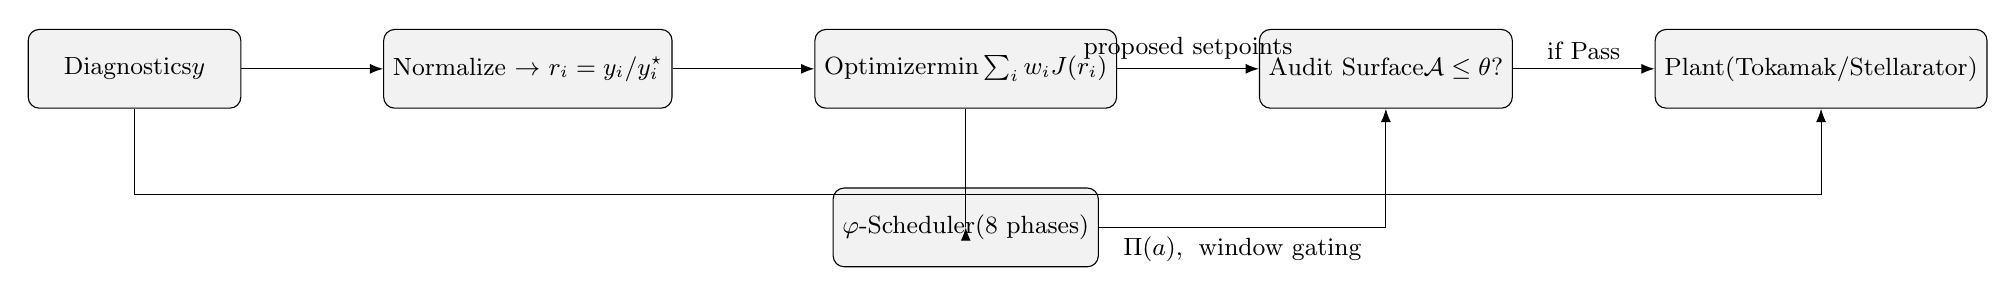
\begin{tikzpicture}[font=\small,node distance=8mm,>=Latex]
\node[draw,rounded corners,minimum width=2.7cm,minimum height=1.0cm,fill=gray!10] (diag) {Diagnostics\\$y$};
\node[draw,rounded corners,minimum width=3.3cm,minimum height=1.0cm,fill=gray!10,right=18mm of diag] (rat) {Normalize $\to$ $r_i=y_i/y_i^\star$};
\node[draw,rounded corners,minimum width=3.2cm,minimum height=1.0cm,fill=gray!10,right=18mm of rat] (opt) {Optimizer\\$\min \sum_i w_i J(r_i)$};
\node[draw,rounded corners,minimum width=3.0cm,minimum height=1.0cm,fill=gray!10,below=10mm of opt] (sched) {$\varphi$-Scheduler\\(8 phases)};
\node[draw,rounded corners,minimum width=3.0cm,minimum height=1.0cm,fill=gray!10,right=18mm of opt] (audit) {Audit Surface\\$\mathcal A\le\theta$?};
\node[draw,rounded corners,minimum width=2.7cm,minimum height=1.0cm,fill=gray!10,right=18mm of audit] (plant) {Plant\\(Tokamak/Stellarator)};

\draw[->] (diag) -- (rat);
\draw[->] (rat) -- (opt);
\draw[->] (opt) -- node[above] {proposed setpoints} (audit);
\draw[->] (audit) -- node[above] {if Pass} (plant);
\draw[->] (opt) |- (sched);
\draw[->] (sched) -| node[pos=0.25,below] {$\Pi(a)$,\; window gating} (audit);
\draw[<-] (plant) |- ++(-1.0,-1.6) -| (diag);
\end{tikzpicture}
\end{center}

\subsection*{Key definitions}
\textbf{Recognition ratios:} $r_i=y_i/y_i^\star$ over declared targets ($T_e,T_i,n_e$, $q$-profile metrics, shear proxy $\gamma_{E\times B}/\gamma^\star$, turbulence bands, impurity/radiated fractions).\\
\textbf{$\varphi$-timed schedule:} $L{=}8$ windows; actuator class assignment $\Pi(a)\subset\{0,\dots,7\}$.\\
\textbf{Audit surface (certificate):} fixed thresholds on disruptivity risk, impurity/radiation fractions, transport proxies, and tracking error; non-passing policies are auto-rejected/filtered.

\subsection*{Best Mode (preferred embodiment)}
\begin{itemize}[leftmargin=1.1em]
\item \textbf{Actuators:} NBI (two phases for torque/shear), ECRH (two phases for core/edge), ICRH (single phase), RMP (single phase), pellets (single phase), gas puffing (single phase), shaping/VS (fast loop; updates gated).
\item \textbf{Diagnostics:} Thomson, ECE, reflectometry, BES, SXR/bolometry, neutron rate, magnetic probes, loop voltage, equilibrium reconstructions.
\item \textbf{Window map:} $\Pi(\text{pellet})=\{0\}$, $\Pi(\text{RMP})=\{2\}$, $\Pi(\text{ECRH})=\{1,5\}$, $\Pi(\text{ICRH})=\{3\}$, $\Pi(\text{NBI})=\{4,7\}$, $\Pi(\text{Gas})=\{6\}$.
\item \textbf{Objective:} $\sum_i w_i J(r_i)$ with $w_i$ set from sensitivity of a certified transport surrogate at $r=1$.
\item \textbf{Controller:} periodic MPC ($N{=}10$--$30$ steps, terminal set/cost 8-phase periodic); fallback RL with safety filter that solves the same constrained ledger problem online.
\item \textbf{Certificate thresholds:} declare fixed $\theta$ for risk, impurities, radiated fraction, and tracking error; deployment only if $\mathcal A\le\theta$ for $M$ consecutive windows.
\end{itemize}

\subsection*{Quick figure: eight-phase $\varphi$ schedule}
\begin{center}
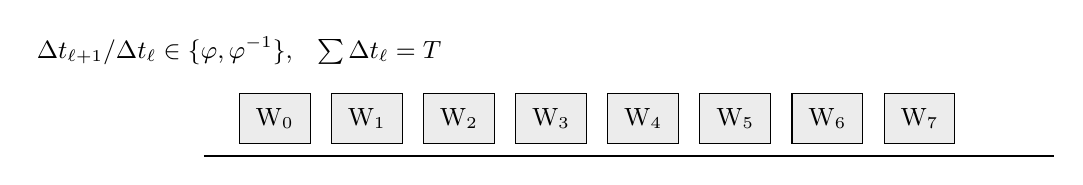
\begin{tikzpicture}[x=0.9cm,y=0.8cm,font=\small]
\draw[thick] (0,0) -- (12,0);
\foreach \i/\lab in {0/W$_0$,1/W$_1$,2/W$_2$,3/W$_3$,4/W$_4$,5/W$_5$,6/W$_6$,7/W$_7$}{
  \pgfmathsetmacro{\x}{0.5+1.3*\i}
  \draw[fill=gray!15] (\x,0.2) rectangle +(1.0,0.8);
  \node at (\x+0.5,0.6) {\lab};
}
\node[above] at (0.5,1.3) {$\Delta t_{\ell+1}/\Delta t_\ell\in\{\varphi,\varphi^{-1}\}$, \; $\sum \Delta t_\ell=T$};
\end{tikzpicture}
\end{center}

\medskip

%======================== SPEC II =========================
\section*{SPEC II — ICF $\varphi$-Pulse Shaping}

\subsection*{Summary}
An ICF pulse-shaping method that constructs $\varphi$-spaced sub-pulses and minimizes a \emph{symmetry ledger} over normalized spherical-harmonic mode magnitudes $r_{\ell m}=|a_{\ell m}|/a^\star_\ell$ subject to energy/facility constraints. Deployment is certificate-gated. Residual asymmetry decreases at least geometrically with sub-pulse count within the admissible regime.

\subsection*{Quick figure: $\varphi$-spaced sub-pulse train}
\begin{center}
\begin{tikzpicture}[x=0.8cm,y=1.0cm,>=Latex,font=\small]
\draw[->] (0,0) -- (12,0) node[right] {$t$};
\foreach \x/\h in {1/1.0,2.6/1.5,4.1/1.2,6.7/1.7,8.0/1.4,10.9/1.8}{
  \draw[thick] (\x,0) -- (\x,\h);
}
\node[below] at (1,0) {$t_1$};
\node[below] at (2.6,0) {$t_2$};
\node[below] at (4.1,0) {$t_3$};
\node[below] at (6.7,0) {$t_4$};
\node[below] at (8.0,0) {$t_5$};
\node[below] at (10.9,0) {$t_6$};
\node[above] at (6,1.9) {$\dfrac{\Delta t_{k+1}}{\Delta t_k}\in\{\varphi,\varphi^{-1}\}$};
\end{tikzpicture}
\end{center}

\subsection*{Key definitions}
\textbf{Symmetry coefficients:} $a_{\ell m}$ from x-ray self-emission, radiography, or backlighter. \\
\textbf{Symmetry ledger:}
$\displaystyle \mathcal L_{\rm sym}=\sum_{\ell\in\mathcal S} w_\ell\sum_{m=-\ell}^{\ell}J\big(|a_{\ell m}|/a^\star_\ell\big)$,
with declared $\mathcal S$ (e.g.\ $\{2,4,6\}$), targets $a^\star_\ell>0$, and weights $w_\ell>0$.\\
\textbf{Certificate:} thresholds on $\mathcal L_{\rm sym}$, mode caps (e.g.\ $|a_{20}|\le\tau_2$, $|a_{4m}|\le\tau_4$), shock timing/bang-time windows, adiabat and preheat limits.

\subsection*{Best Mode (preferred embodiment)}
\begin{itemize}[leftmargin=1.1em]
\item \textbf{Sub-pulses:} $K=5$--$8$ pickets/ramps with raised-cosine template $s(\cdot)$; amplitudes $A_k$ bounded by facility cone/ring allocations; total energy $E_{\rm tot}$ fixed.
\item \textbf{Timing:} enforce $\Delta t_{k+1}/\Delta t_k\in\{\varphi,\varphi^{-1}\}$ within a declared drive window; per-ring micro-delays allowed if $\varphi$-commensurability preserved.
\item \textbf{Mode set:} $\mathcal S=\{2,4,6\}$ with $a^\star_\ell$ set from prior symmetry campaigns; $w_\ell$ proportional to capsule-yield sensitivity.
\item \textbf{Optimizer:} hydrodynamics surrogate with declared error bounds; optionally Bayesian update from low-energy surrogate shots; keep ledger, $\varphi$-spacing, and certificate fixed.
\item \textbf{On-shot gating:} online symmetry proxies checked; certificate violation aborts remaining sub-pulses.
\end{itemize}

\medskip

%======================== SPEC III =========================
\section*{SPEC III — $\varphi$-Scheduler Module}

\subsection*{Summary}
A reusable scheduling module that partitions control periods into $\varphi$-commensurate windows, assigns actuators to phase sets, enforces update admissibility within windows, guarantees periodic invariance with bounded jitter, provides a qualitative interference bound, and exposes a controller-agnostic \emph{Compliance API} with signed logs. Useful across domains (fusion, lasers, robotics, beamlines, power electronics).

\subsection*{Quick figure: scheduler architecture \& API}
\begin{center}
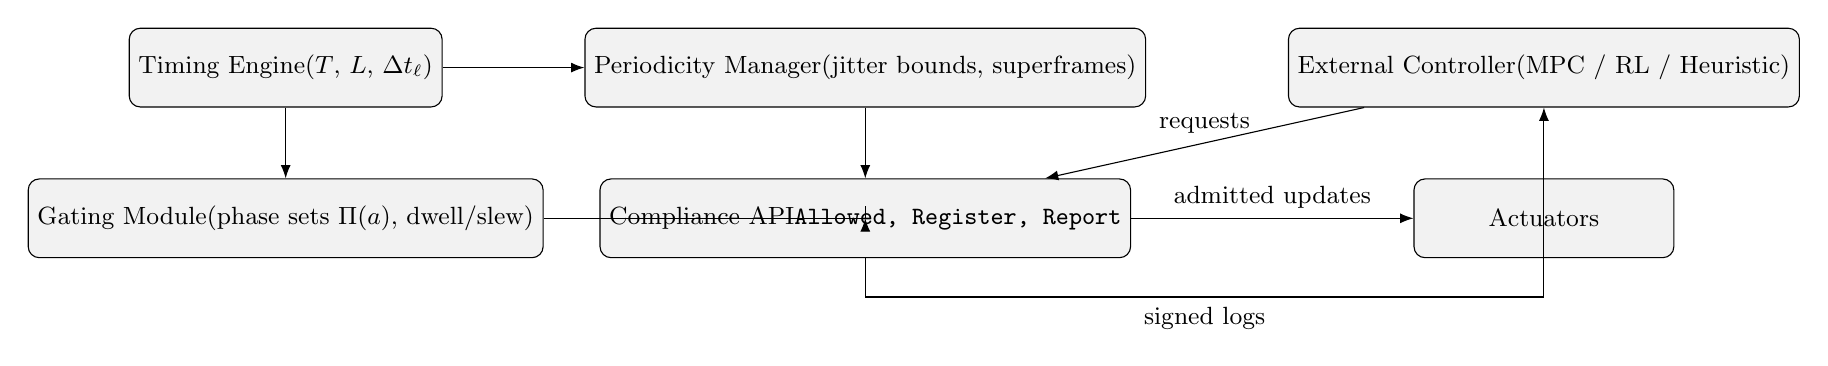
\begin{tikzpicture}[font=\small,node distance=9mm,>=Latex]
\node[draw,rounded corners,fill=gray!10,minimum width=3.6cm,minimum height=1.0cm] (tim) {Timing Engine\\($T$, $L$, $\Delta t_\ell$)};
\node[draw,rounded corners,fill=gray!10,minimum width=3.6cm,minimum height=1.0cm,below=of tim] (gate) {Gating Module\\(phase sets $\Pi(a)$, dwell/slew)};
\node[draw,rounded corners,fill=gray!10,minimum width=3.6cm,minimum height=1.0cm,right=18mm of tim] (per) {Periodicity Manager\\(jitter bounds, superframes)};
\node[draw,rounded corners,fill=gray!10,minimum width=3.6cm,minimum height=1.0cm,below=of per] (api) {Compliance API\\\texttt{Allowed, Register, Report}};
\node[draw,rounded corners,fill=gray!10,minimum width=3.3cm,minimum height=1.0cm,right=18mm of per] (ctrl) {External Controller\\(MPC / RL / Heuristic)};
\node[draw,rounded corners,fill=gray!10,minimum width=3.3cm,minimum height=1.0cm,below=of ctrl] (act) {Actuators};

\draw[->] (tim) -- (gate);
\draw[->] (tim) -- (per);
\draw[->] (gate) -| (api);
\draw[->] (per) -- (api);
\draw[->] (ctrl) -- node[above] {requests} (api);
\draw[->] (api) -- node[above] {admitted updates} (act);
\draw[->] (api) |- ++(0,-1.0) -| node[pos=0.25,below] {signed logs} (ctrl);
\end{tikzpicture}
\end{center}

\subsection*{Key definitions}
\textbf{$\varphi$-windows:} $L{=}8$ default; optional superframe $S\,T$ with $\varphi$-relations preserved inside each $T$. \\
\textbf{Interference bound (qualitative):} For band-limited cross-coupling, time-averaged bilinear cross-terms are reduced by a strict factor $\kappa\in(0,1)$ relative to co-phased/equal-spaced baselines (window smoothness controls $\kappa$).\\
\textbf{Compliance API:} \texttt{BeginWindow($\ell$)}, \texttt{EndWindow($\ell$)}, \texttt{WindowIndex()}, \texttt{Allowed($a$)}, \texttt{RequestUpdate($a$,payload)} (admit/reject), \texttt{GetComplianceReport()} (cryptographically signed).

\subsection*{Best Mode (preferred embodiment)}
\begin{itemize}[leftmargin=1.1em]
\item \textbf{Timing:} $T$ linked to plant reference $\tau_{\rm ref}$; $L{=}8$; raised-cosine window edges; jitter $\le$ 100~$\mu$s (magnetic) / 100~ps (ICF triggers).
\item \textbf{Phase sets:} disjoint or minimally overlapping $\Pi(a)$ for actuators with strong cross-coupling; mandatory dwell $\delta_a$ enforced.
\item \textbf{Compliance:} hardware timer/FPGA for edges; secure element for signature of logs; per-period attestation of $\varphi$-ratios and window adherence.
\item \textbf{Integration:} controller-agnostic; third-party stacks must call API; noncompliant requests are rejected and logged.
\end{itemize}

\bigskip

%======================== OPTIONAL CLAIMS OUTLINE =========================
\section*{Claims (outline — each spec provides an independent set)}
\begin{itemize}[leftmargin=1.1em]
\item \textbf{Spec I (Magnetic Controller):} Method, System, and Non-transitory Medium claims covering ledger-objective over recognition ratios, $\varphi$-timed eight-phase actuation with assignments $\Pi(a)$, certificate-gated deployment, periodic MPC or RL with safety filter; dependent claims on actuators, diagnostics, specific ratios (critical gradients, shear), periodic terminal ingredients, robustness bounds.
\item \textbf{Spec II (ICF $\varphi$-Pulse Shaper):} Method, System, and Medium claims covering $\varphi$-spaced sub-pulses, symmetry-ledger minimization over $|a_{\ell m}|/a^\star_\ell$, certificate thresholds, and a geometric convergence feature ($0<\eta<1$ qualitative); dependent claims on pulse templates, mode sets, facility constraints, online gating.
\item \textbf{Spec III ($\varphi$-Scheduler):} Method, System, and Medium claims covering $\varphi$-commensurate windows, periodic invariance and interference bounds, and the Compliance API with signed logs; dependent claims on jitter bounds, superframes, window smoothness, hardware realization.
\end{itemize}

\bigskip

%======================== ENABLEMENT CHECKLIST =========================
\section*{Enablement \& best-mode checklist (for counsel)}
\begin{itemize}[leftmargin=1.1em]
\item Equations/algorithms present (ledger $J$, ratios $r$, $\varphi$-windowing; symmetry ledger). 
\item Concrete mappings (actuator phase sets; pulse timing; API calls). 
\item Figures showing pipeline, schedule, pulse train, and module blocks.
\item Best Mode sections for each spec: actuators/diagnostics \& thresholds; $K$ sub-pulses \& mode set; timing/jitter \& API/signing.
\end{itemize}

\end{document}
